\documentclass[tikz,border=3mm]{standalone}

\usepackage{amsmath}
\usepackage{xcolor}
\usetikzlibrary{positioning,fit,backgrounds,arrows.meta}

% 색 정의: 네 포스터 색과 비슷하게 임시 정의
\definecolor{snunavy}{HTML}{1F4E79}
\definecolor{snunavy2}{HTML}{2F6690}
\definecolor{snulight}{HTML}{EAF2F8}
\definecolor{snulight2}{HTML}{F4F8FB}
\definecolor{accentred2}{HTML}{B94A48}
\definecolor{accentredlight}{HTML}{FBEAEA}
\definecolor{textgray}{HTML}{444444}

\begin{document}

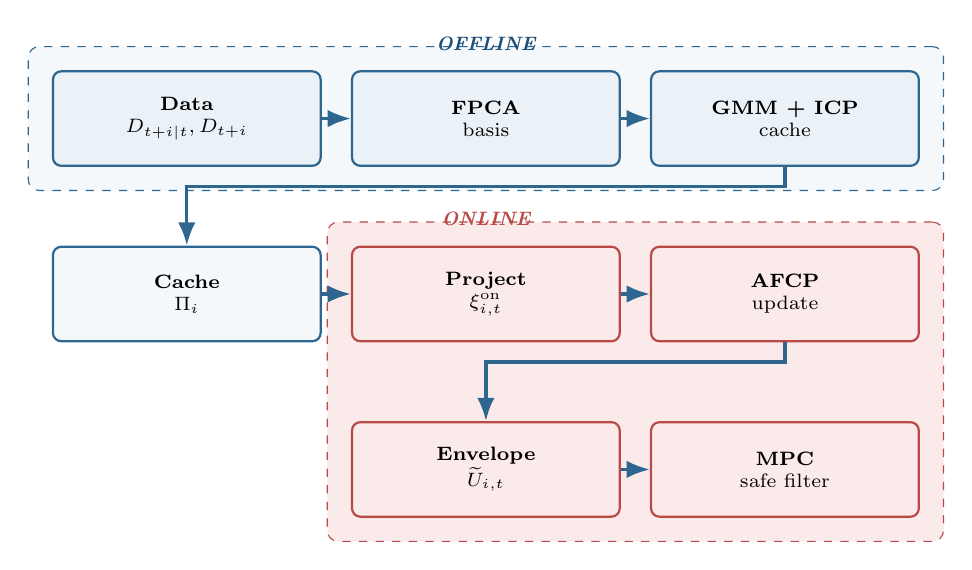
\begin{tikzpicture}[
  node distance=2.7mm and 3.7mm,
  every node/.style={font=\scriptsize},
  blockA/.style={
    rectangle,rounded corners=3pt,draw=snunavy2,thick,
    fill=snulight,align=center,
    minimum width=34mm,minimum height=12mm,inner sep=1.8pt
  },
  blockB/.style={
    rectangle,rounded corners=3pt,draw=accentred2,thick,
    fill=accentredlight,align=center,
    minimum width=34mm,minimum height=12mm,inner sep=1.8pt
  },
  arrow/.style={-Latex,very thick,snunavy2},
  label/.style={font=\scriptsize\itshape,text=textgray},
]
\node[blockA] (cal) {\textbf{Data}\\$D_{t+i\mid t},D_{t+i}$};
\node[blockA,right=of cal] (fpca) {\textbf{FPCA}\\basis};
\node[blockA,right=of fpca] (gmm) {\textbf{GMM + ICP}\\cache};
\node[label,above=1.3mm of fpca]
  {\textcolor{snunavy}{\bfseries OFFLINE}};
\draw[arrow] (cal) -- (fpca);
\draw[arrow] (fpca) -- (gmm);

\node[blockA,below=10mm of cal,fill=snulight2] (cache)
  {\textbf{Cache}\\$\Pi_i$};
\draw[arrow] (gmm.south) -- ++(0,-2.5mm) -| (cache.north);

\node[blockB,right=of cache] (proj)
  {\textbf{Project}\\$\xi^{\mathrm{on}}_{i,t}$};
\node[blockB,right=of proj] (afcp)
  {\textbf{AFCP}\\update};
\draw[arrow] (cache) -- (proj);
\draw[arrow] (proj) -- (afcp);

\node[blockB,below=10mm of proj] (env)
  {\textbf{Envelope}\\$\widetilde U_{i,t}$};
\node[blockB,right=of env] (mpc)
  {\textbf{MPC}\\safe filter};
\draw[arrow] (afcp.south) -- ++(0,-2.5mm) -| (env.north);
\draw[arrow] (env) -- (mpc);

\node[label,above=1.3mm of proj]
  {\textcolor{accentred2}{\bfseries ONLINE}};

\begin{pgfonlayer}{background}
  \node[fit=(cal)(gmm),fill=snulight2,rounded corners,
        inner sep=3mm,draw=snunavy2,dashed] {};
  \node[fit=(proj)(afcp)(env)(mpc),fill=accentredlight,rounded corners,
        inner sep=3mm,draw=accentred2,dashed] {};
\end{pgfonlayer}
\end{tikzpicture}

\end{document}